\documentclass[10pt, landscape]{article}
\usepackage[scaled=0.92]{helvet}
\usepackage{calc}
\usepackage{multicol}
\usepackage[a4paper,margin=3mm,landscape]{geometry}
\usepackage{amsmath,amsthm,amsfonts,amssymb}
\usepackage{color,graphicx,overpic}
\usepackage{hyperref}
\usepackage{newtxtext} 
\usepackage{enumitem}
\usepackage[table]{xcolor}
\usepackage{mathtools}
% for drawing diragrams/graphs
\usepackage{tikz}
\usetikzlibrary{arrows.meta}
\usetikzlibrary{calc}
\setlist{nosep}

% ADDITIONAL USEFUL PACKAGES:
% for matrices
\usepackage{nicematrix}
% for relations
\usepackage{cancel}
\usepackage{ mathrsfs }
% for including images
\graphicspath{ {./images/} }


\pdfinfo{
  /Title (CS2102 ER Models with Relational Schema.pdf)
  /Creator (TeX)
  /Producer (pdfTeX 1.40.0)
  /Author (Jovyn Tan)
  /Subject (CS2102)
/Keywords (CS2102,dbms,rdbms,database,nus,cheatsheet,pdf)}

% Turn off header and footer
\pagestyle{empty}

% redefine section commands to use less space
\makeatletter
\renewcommand{\section}{\@startsection{section}{1}{0mm}%
  {-1ex plus -.5ex minus -.2ex}%
  {0.5ex plus .2ex}%x
{\normalfont\large\bfseries}}
\renewcommand{\subsection}{\@startsection{subsection}{2}{0mm}%
  {-1explus -.5ex minus -.2ex}%
  {0.5ex plus .2ex}%
{\normalfont\normalsize\bfseries}}
\renewcommand{\subsubsection}{\@startsection{subsubsection}{3}{0mm}%
  {-1ex plus -.5ex minus -.2ex}%
  {1ex plus .2ex}%
{\normalfont\small\bfseries}}%
\makeatother

\renewcommand{\familydefault}{\sfdefault}
\renewcommand\rmdefault{\sfdefault}
%  makes nested numbering (e.g. 1.1.1, 1.1.2, etc)
\renewcommand{\labelenumii}{\theenumii}
\renewcommand{\theenumii}{\theenumi.\arabic{enumii}.}
\renewcommand\labelitemii{•}

\definecolor{mathblue}{cmyk}{1,.72,0,.38}
\everymath\expandafter{\the\everymath \color{mathblue}}

% Don't print section numbers
\setcounter{secnumdepth}{0}

\setlength{\parindent}{0pt}
\setlength{\parskip}{0pt plus 0.5ex}
%% this changes all items (enumerate and itemize)
\setlength{\leftmargini}{0.5cm}
\setlength{\leftmarginii}{0.5cm}
\setlist[itemize,1]{leftmargin=2mm,labelindent=1mm,labelsep=1mm}
\setlist[itemize,2]{leftmargin=4mm,labelindent=1mm,labelsep=1mm}

% adding my commands
% tightcenter
\newenvironment{tightcenter}{%
  \setlength\topsep{0pt}
  \setlength\parskip{0pt}
  \begin{center}
    }{%
  \end{center}
}

% boxed
\newenvironment{tightbox}{%
  \setlength\topsep{0pt}
  \setlength\parskip{0pt}
  \begin{center}
    \begin{tabular}{|@{\hspace{\dimexpr\fboxsep+0.5\arrayrulewidth}}c@{\hspace{\dimexpr\fboxsep+0.5\arrayrulewidth}}|}
      \hline
    }
    {%
    \\ \hline
    \end{tabular}
  \end{center}
}

% fixed width box
\newenvironment{fixedbox}[1][0.7]{
  \setlength\topsep{0pt}
  \setlength\parskip{0pt}
  \begin{center}
    \begin{tabular}{|>{\centering\arraybackslash}m{#1\linewidth}|}
    \hline
  }{
  \\ \hline
  \end{tabular}
  \end{center}
}

% definition of a new term
\usepackage{soul}
\definecolor{paleyellow}{RGB}{251,243,218}
\newcommand{\definition}[2][]{\sethlcolor{paleyellow}\hl{\textbf{#2}} #1  $\rightarrow$}

% important note (attention)
\newcommand{\attention}{{\color{red}\textbf{! }}}


\usepackage{color, soul}
\definecolor{lightgray}{gray}{0.9}

\newcommand{\code}[1]{\texttt{\sethlcolor{lightgray}\hl{$\,$#1$\,$}}}
% -----------------------------------------------------------------------

\begin{document}
\raggedright
\footnotesize
\begin{center}
  \fbox{%
    \parbox{0.4\linewidth}{\centering \textcolor{black}{
        {\Large\textbf{CS2102 ER Models \& Relational Schemas}}
      \\ \normalsize{AY21/22 SEM 1}} $\cdot$ {\footnotesize \textcolor{gray}{github/jovyntls}}
    }%
  }
\end{center}

\begin{multicols*}{3}

  % multicol parameters
  % These lengths are set only within the two main columns
  \setlength{\columnseprule}{0.25pt}
  \setlength{\premulticols}{1pt}
  \setlength{\postmulticols}{1pt}
  \setlength{\multicolsep}{1pt}
  \setlength{\columnsep}{2pt}

  \section{AGGREGATION}
  \begin{tightcenter}
    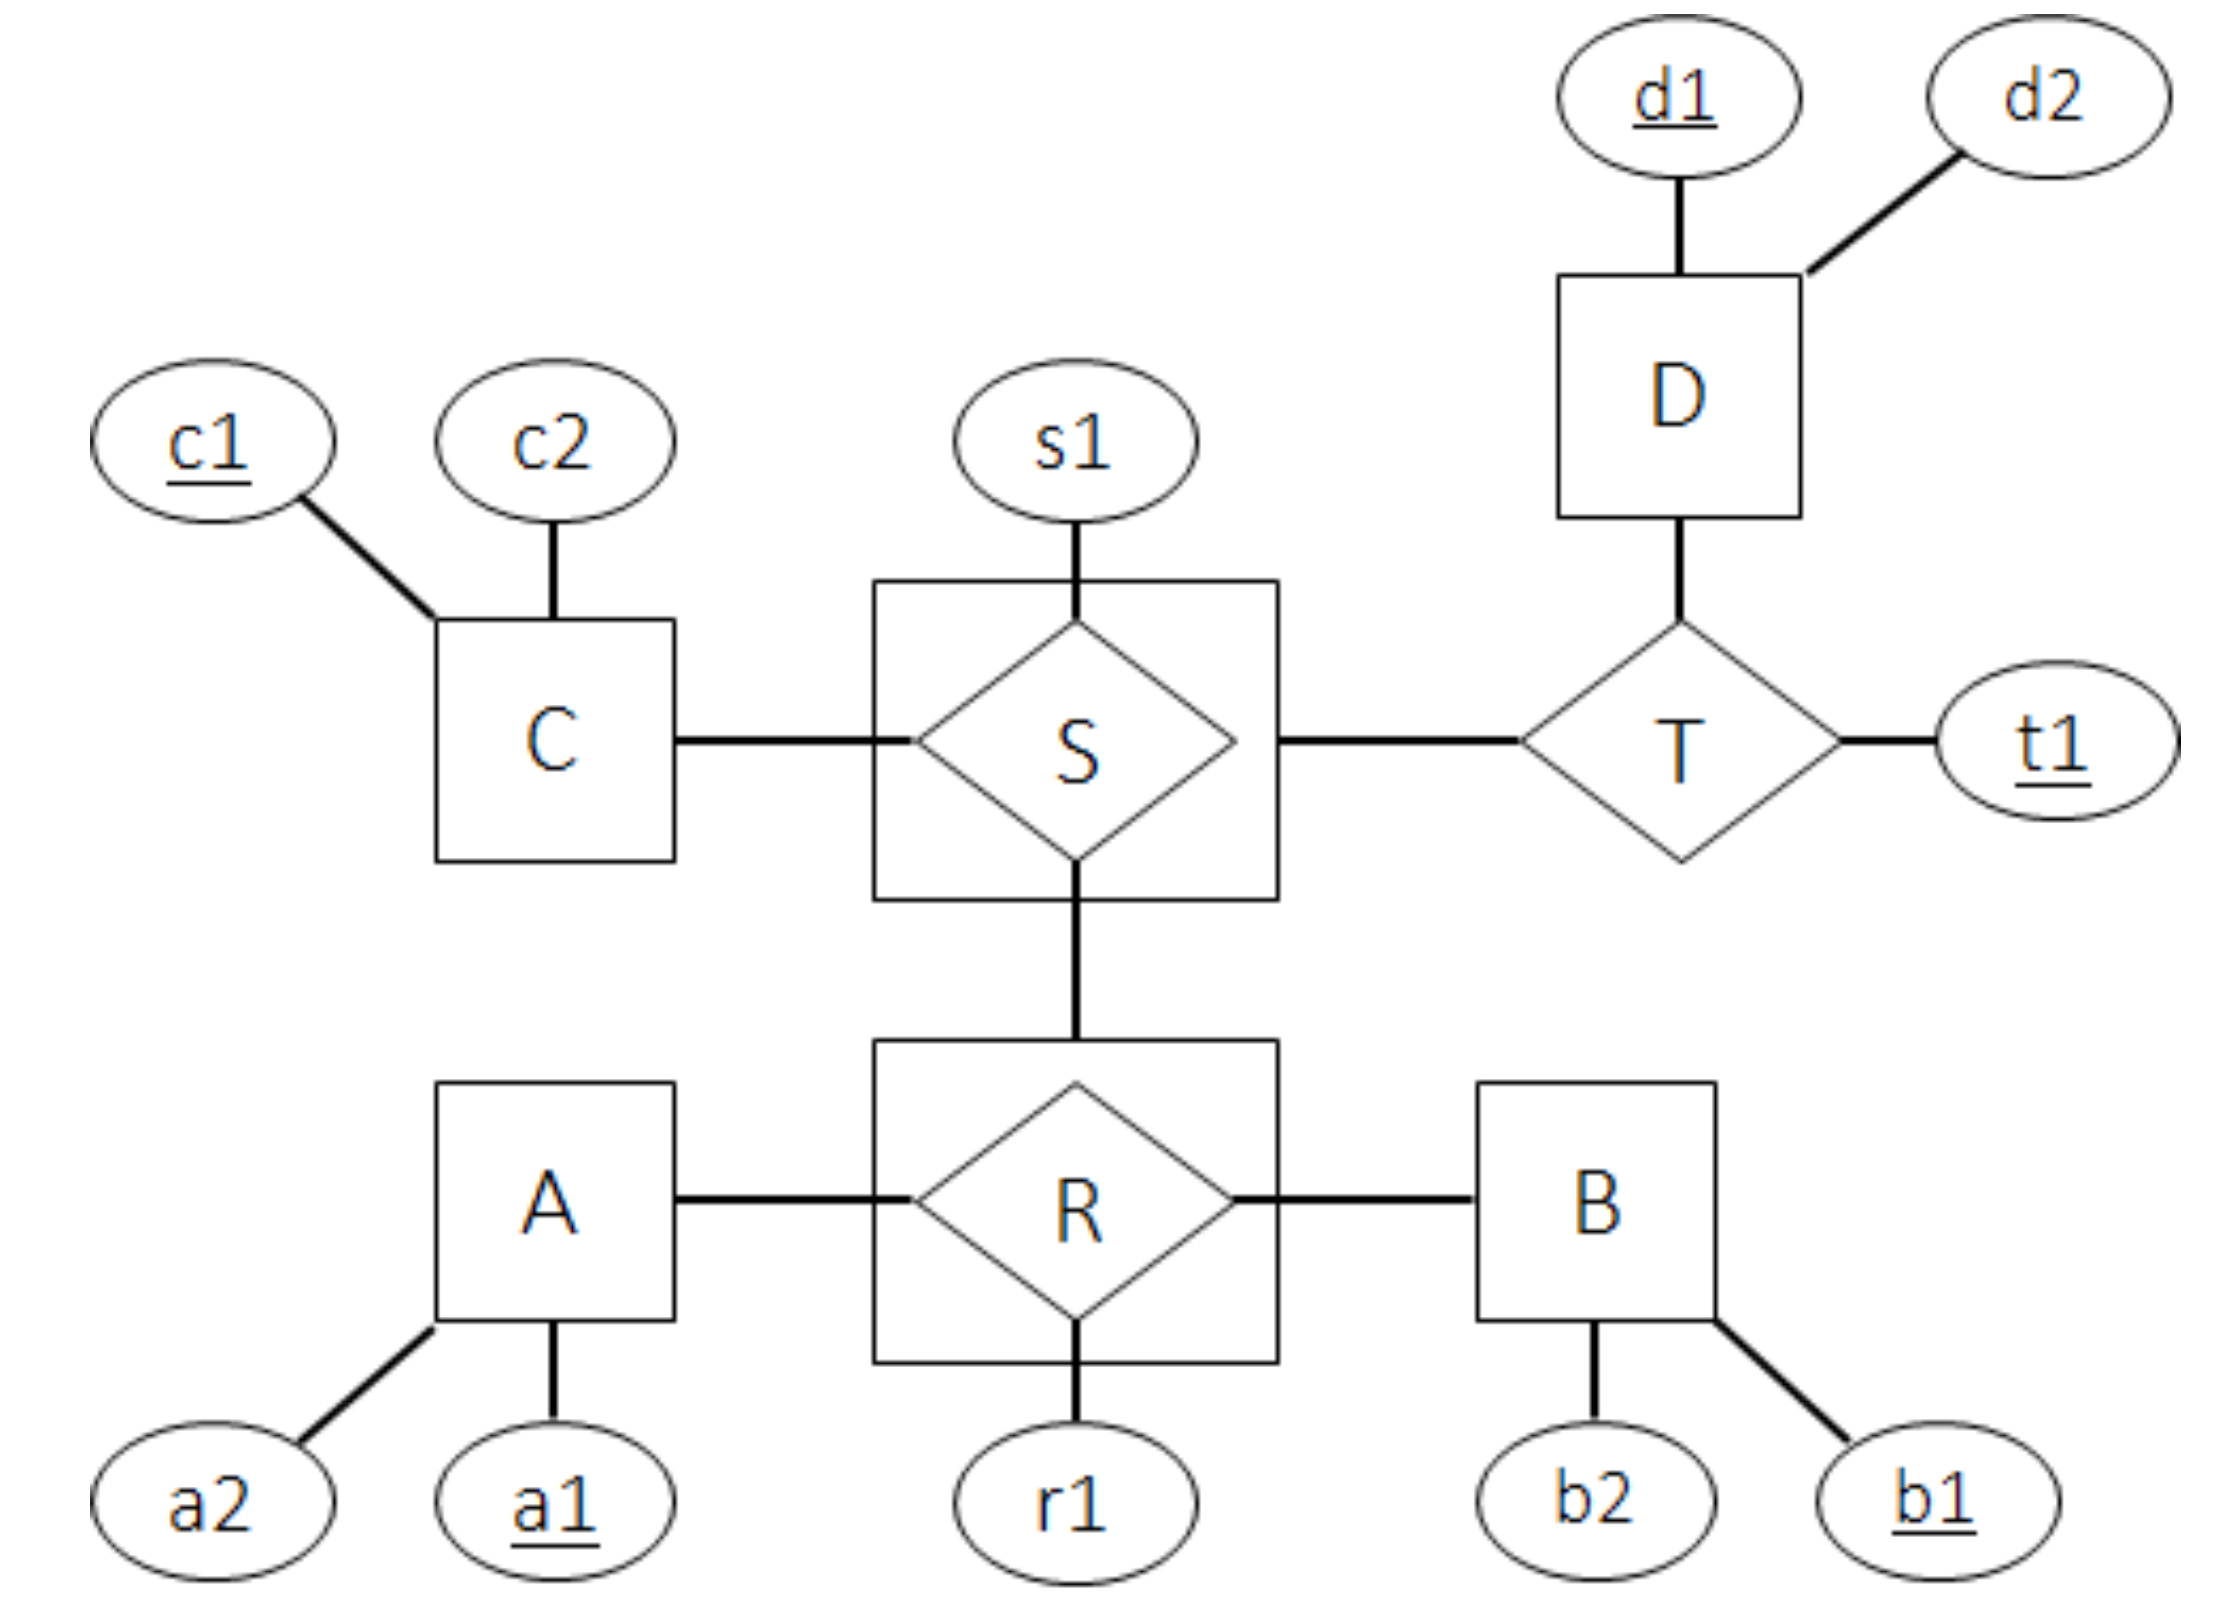
\includegraphics[width=0.85\linewidth]{cs2102-er-model-aggregation.png} 
  \end{tightcenter}
  \begin{lstlisting}[style=mySQL]
DROP TABLE IF EXISTS A, B, C, D, R, S, T CASCADE;
CREATE TABLE A (
  a1 INTEGER PRIMARY KEY,
  a2 INTEGER
);

CREATE TABLE B (
  b1 INTEGER PRIMARY KEY,
  b2 INTEGER
);

CREATE TABLE C (
  c1 INTEGER PRIMARY KEY,
  c2 INTEGER
);

CREATE TABLE D (
  d1 INTEGER PRIMARY KEY,
  d2 INTEGER 
);

CREATE TABLE R (
  a1 INTEGER REFERENCES A, 
  b1 INTEGER REFERENCES B,
  r1 INTEGER,
  PRIMARY KEY (a1, b1) 
);

CREATE TABLE S ( a1 INTEGER,
  b1 INTEGER,
  c1 INTEGER REFERENCES C,
  s1 INTEGER,
  PRIMARY KEY (a1, b1, c1),
  FOREIGN KEY (a1, b1) REFERENCES R
);

CREATE TABLE T (
  a1 INTEGER,
  b1 INTEGER,
  c1 INTEGER,
  d1 INTEGER REFERENCES D,
  t1 INTEGER,
  PRIMARY KEY (a1, b1, c1, d1, t1), 
  FOREIGN KEY (a1, b1, c1) REFERENCES S
);
  \end{lstlisting}

  \section{IS-A}
  \begin{tightcenter}
    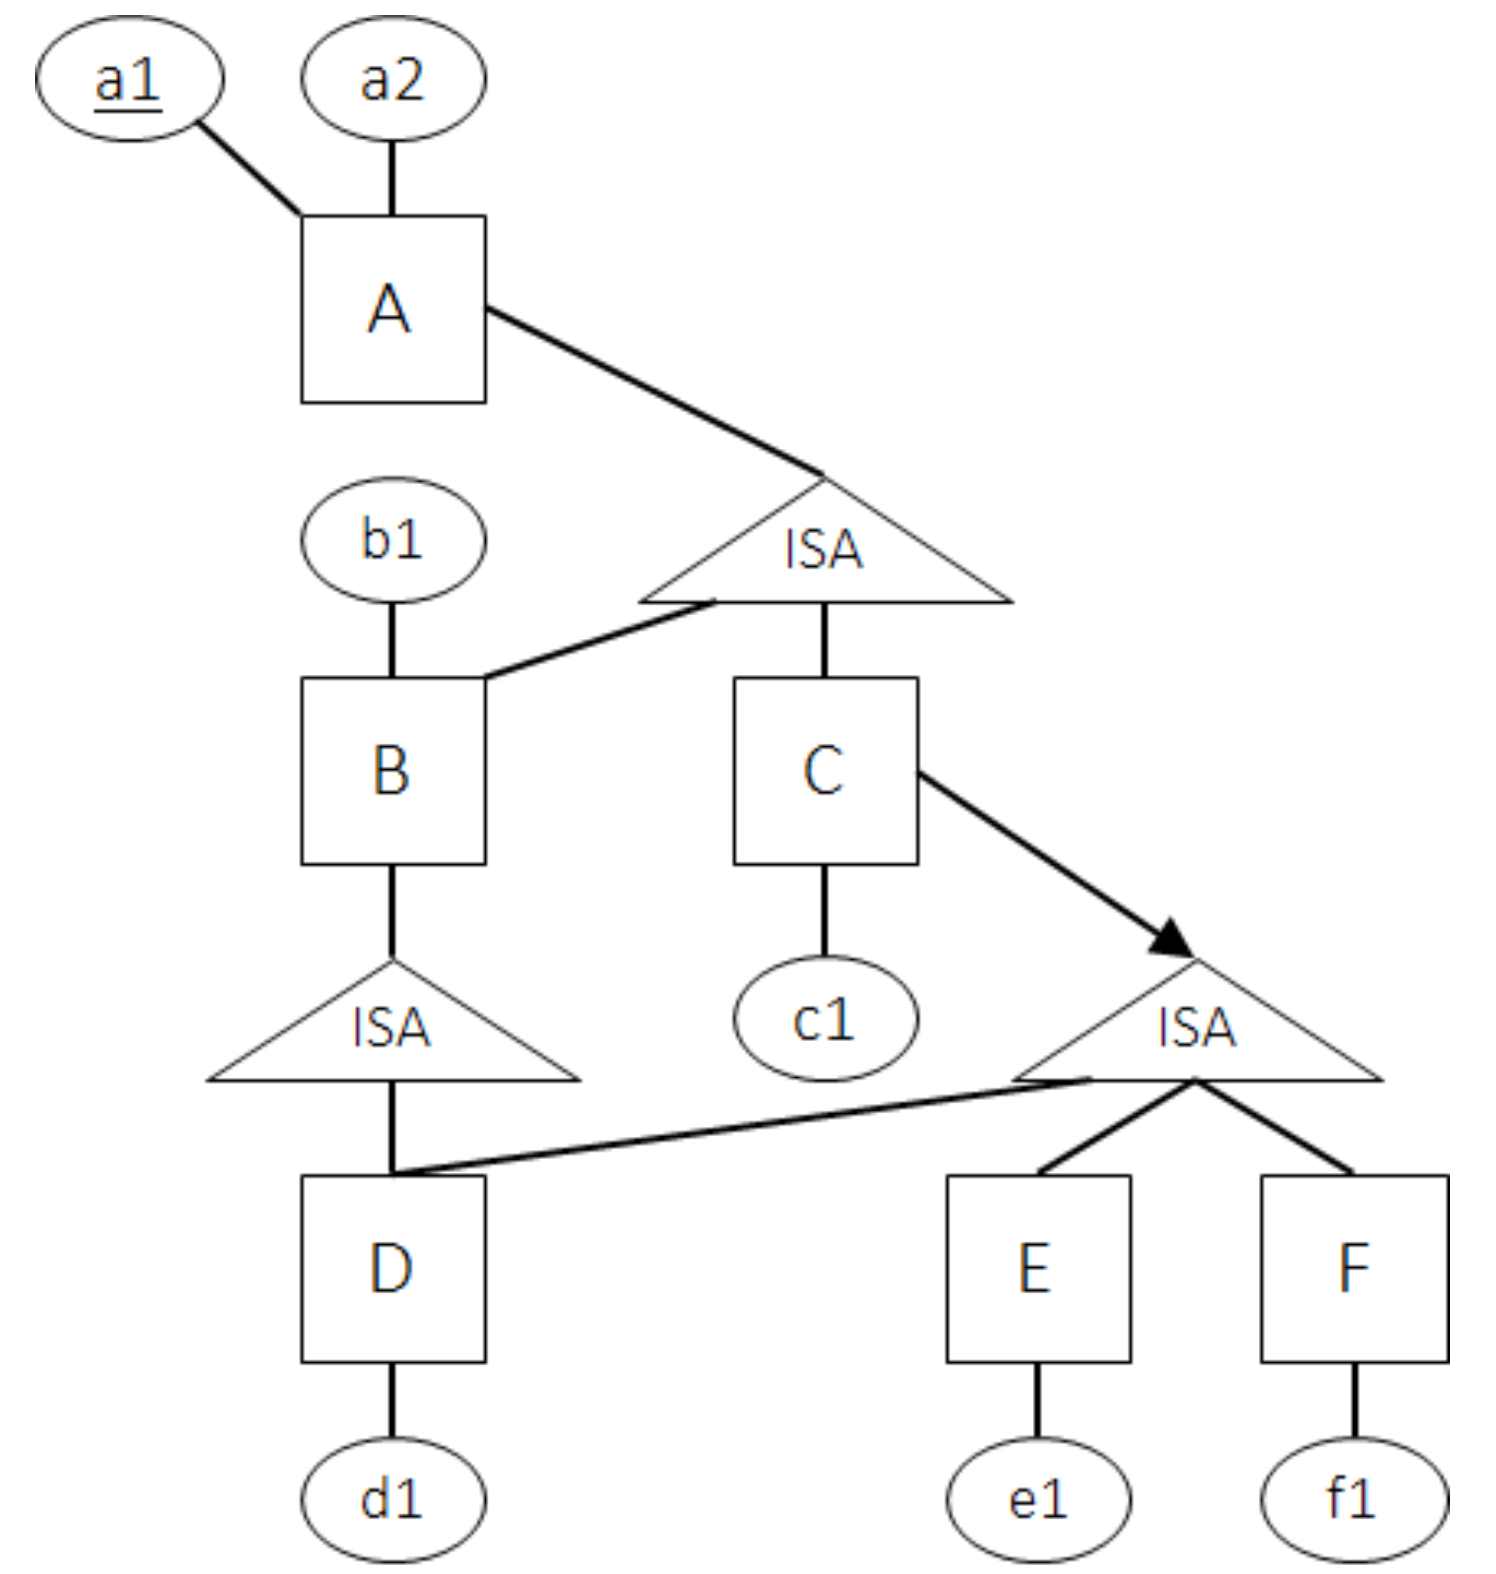
\includegraphics[width=0.8\linewidth]{cs2102-er-model-isa.png} 
  \end{tightcenter}
  \begin{lstlisting}[style=mySQL]
DROP TABLE IF EXISTS A, B, C, D, E, F CASCADE;
CREATE TABLE A (
  a1 INTEGER PRIMARY KEY,
  a2 INTEGER
);

CREATE TABLE B (
  a1 INTEGER PRIMARY KEY REFERENCES A ON DELETE CASCADE,
  b1 INTEGER 
);

CREATE TABLE C (
  a1 INTEGER PRIMARY KEY REFERENCES A ON DELETE CASCADE, 
  c1 INTEGER
);

CREATE TABLE D (
  a1 INTEGER PRIMARY KEY REFERENCES B REFERENCES C ON DELETE CASCADE,
  d1 INTEGER 
);

CREATE TABLE E (
  a1 INTEGER PRIMARY KEY REFERENCES C
  ON DELETE CASCADE, e1 INTEGER
);

CREATE TABLE F (
  a1 INTEGER PRIMARY KEY REFERENCES C
  ON DELETE CASCADE, f1 INTEGER
);
  \end{lstlisting}

  \section{WEAK ENTITY}
  \begin{tightcenter}
    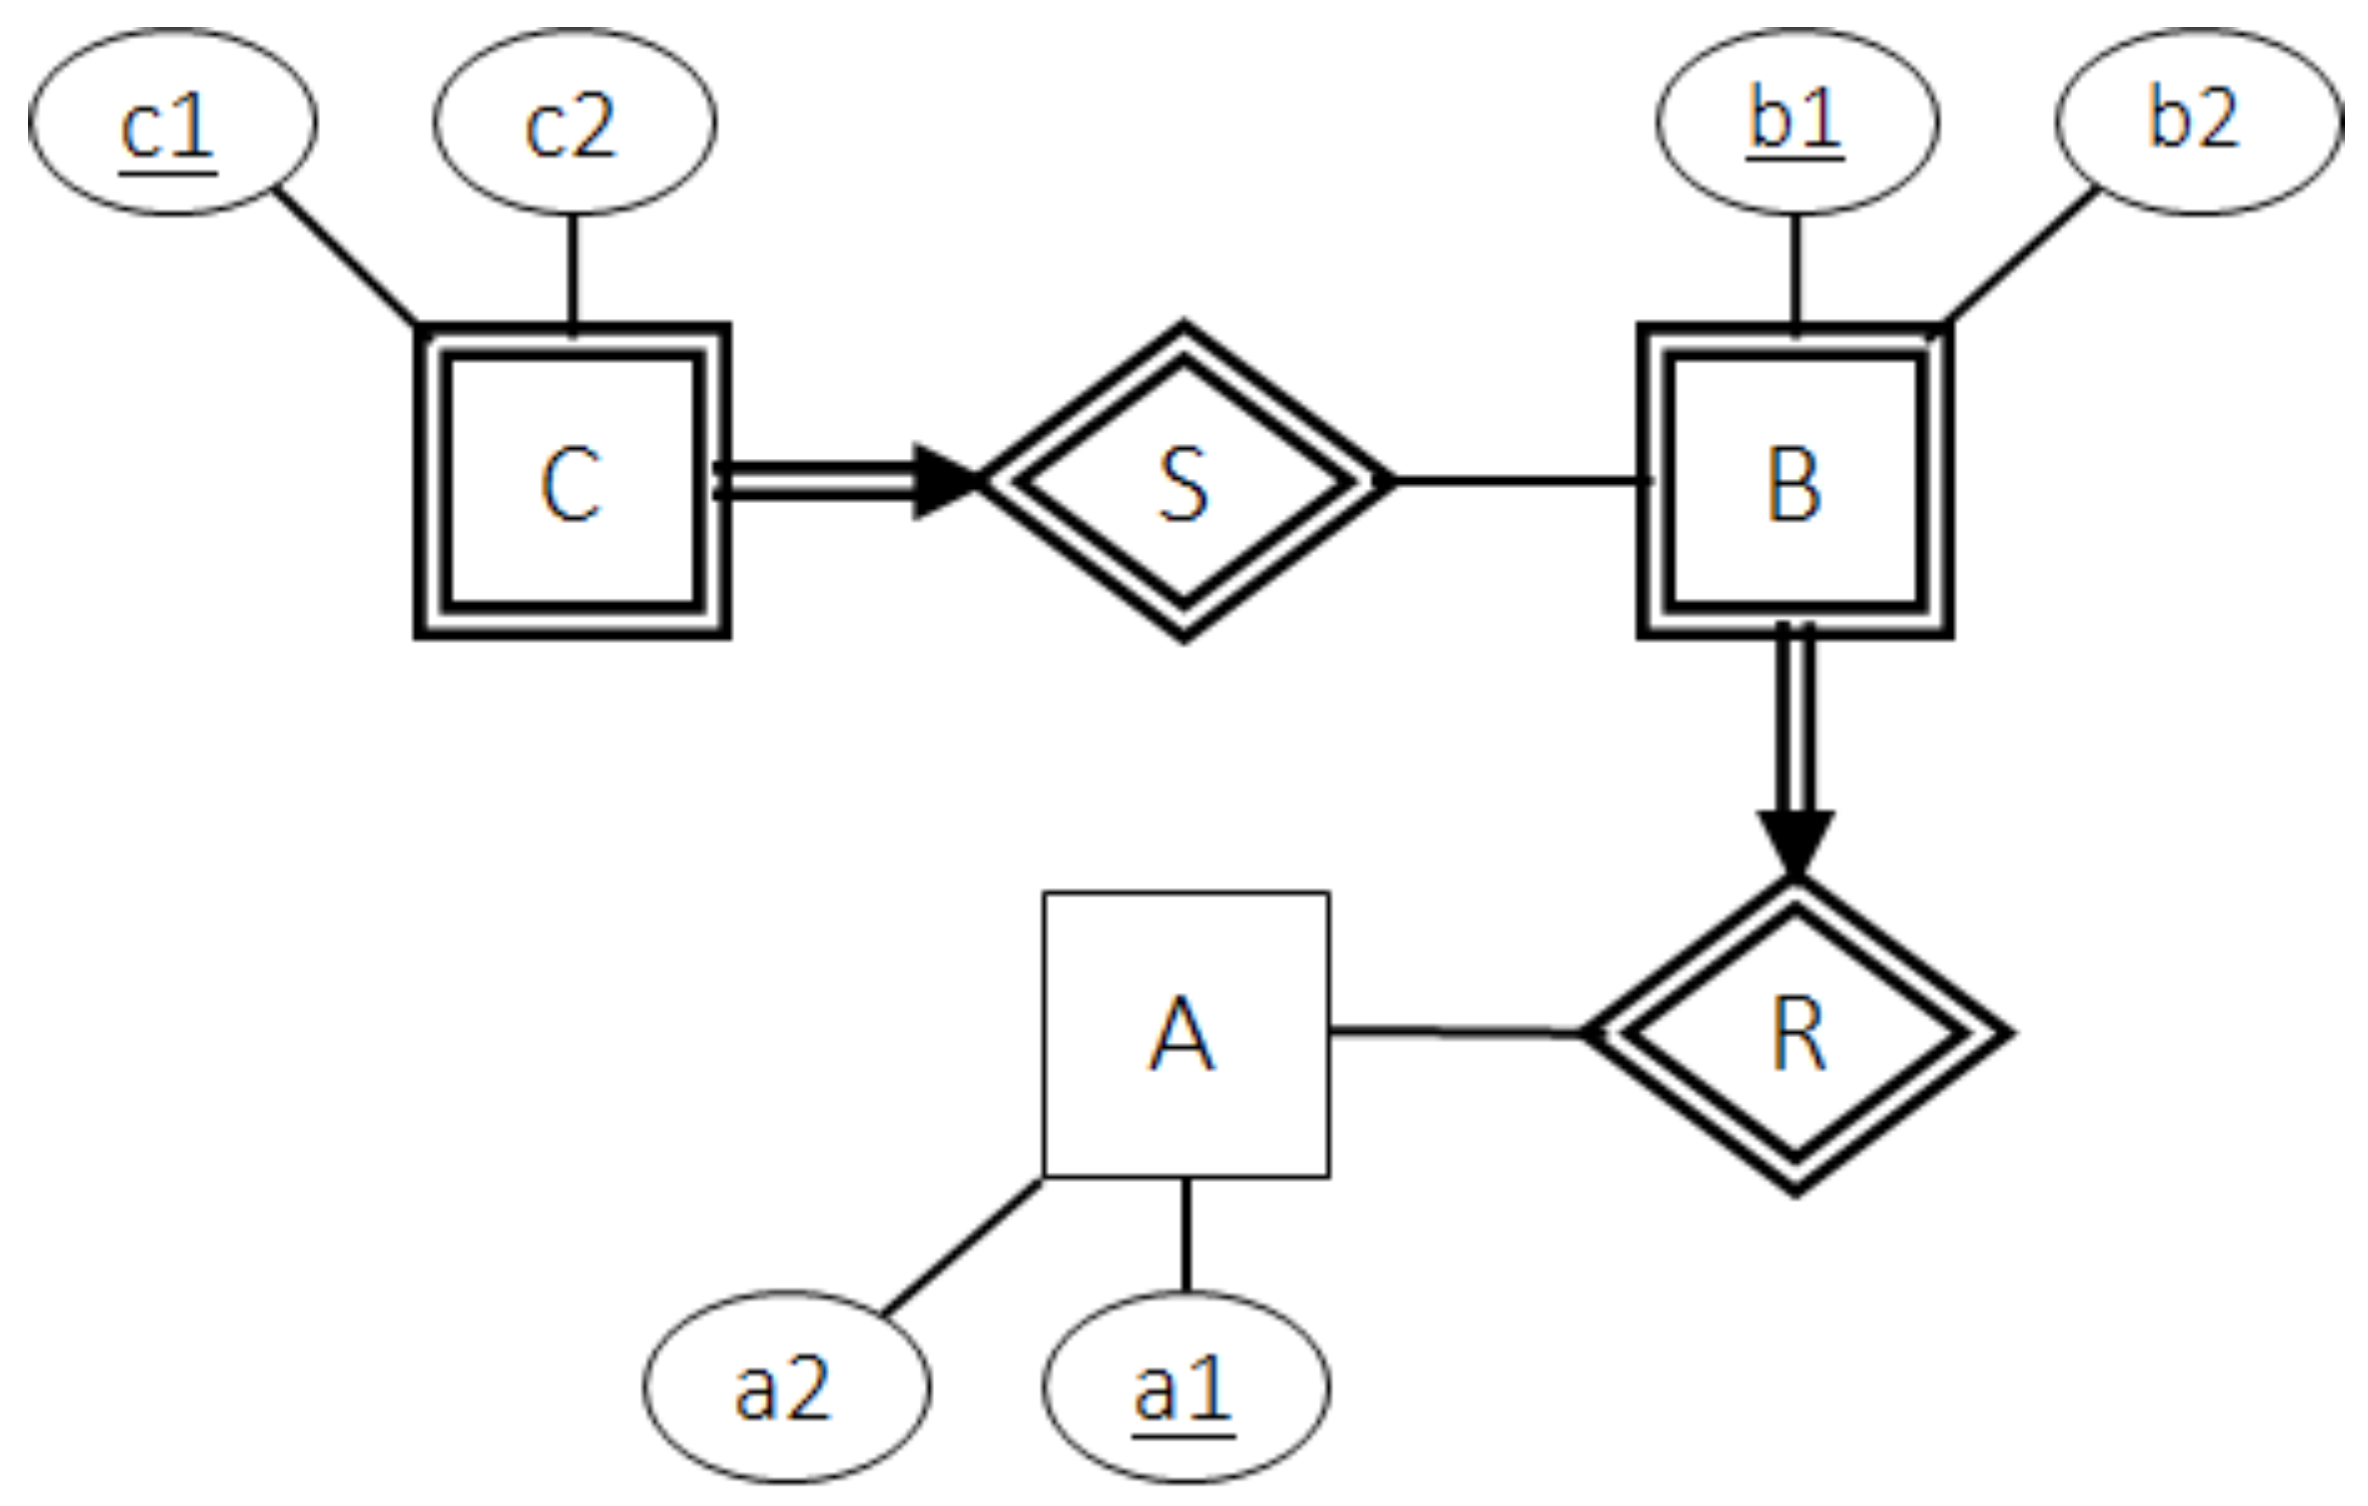
\includegraphics[width=0.9\linewidth]{cs2102-er-model-weak-entity.png} 
  \end{tightcenter}
  \begin{lstlisting}[style=mySQL]
DROP TABLE IF EXISTS A, B, C CASCADE;
CREATE TABLE A (
  a1 INTEGER PRIMARY KEY,
  a2 INTEGER 
);

CREATE TABLE B (
  a1 INTEGER REFERENCES A ON DELETE CASCADE,
  b1 INTEGER,
  b2 INTEGER,
  PRIMARY KEY (a1, b1) 
);

CREATE TABLE C ( 
  a1 INTEGER, 
  b1 INTEGER,
  c1 INTEGER,
  c2 INTEGER,
  PRIMARY KEY (a1, b1, c1),
  FOREIGN KEY (a1, b1) REFERENCES B ON DELETE CASCADE
);
  \end{lstlisting}

\end{multicols*}
\end{document}
